\documentclass[newPxFont,numfooter,sectionpages]{beamer}
\usepackage[utf8]{inputenc}
\usepackage{hyperref}
\hypersetup{colorlinks=true, urlcolor=blue}
\usetheme{sthlm}
\usepackage{pgfplots}
\pgfplotsset{compat=1.14}
\usepackage{cancel}

%-=-=-=-=-=-=-=-=-=-=-=-=-=-=-=-=-=-=-=-=-=-=-=-=
%
%	PRESENTATION INFORMATION
%
%-=-=-=-=-=-=-=-=-=-=-=-=-=-=-=-=-=-=-=-=-=-=-=-=

\title{Bayesian estimation of time-trees:}
\subtitle{A journey through a strange land}
% \date{\today}
\author{Luiz Max Carvalho}
\institute{Postgraduate Symposium 2017\\ Institute of Evolutionary Biology }

\hypersetup{
pdfauthor = {LMCarvalho: lm.carvalho@ed.ac.uk},
pdfsubject = {MCMC},
pdfkeywords = {Bayesian statistics, phylogenetics, MCMC},
pdfmoddate= {D:\pdfdate},
pdfcreator = {}
}

\begin{document}

%-=-=-=-=-=-=-=-=-=-=-=-=-=-=-=-=-=-=-=-=-=-=-=-=
%
%	TITLE PAGE
%
%-=-=-=-=-=-=-=-=-=-=-=-=-=-=-=-=-=-=-=-=-=-=-=-=

\maketitle

%-=-=-=-=-=-=-=-=-=-=-=-=-=-=-=-=-=-=-=-=-=-=-=-=
%	FRAME: Acks
%-=-=-=-=-=-=-=-=-=-=-=-=-=-=-=-=-=-=-=-=-=-=-=-=
\begin{frame}{Acknowledgements}
\begin{columns}
\begin{column}{0.3\textwidth}
    \begin{figure}
     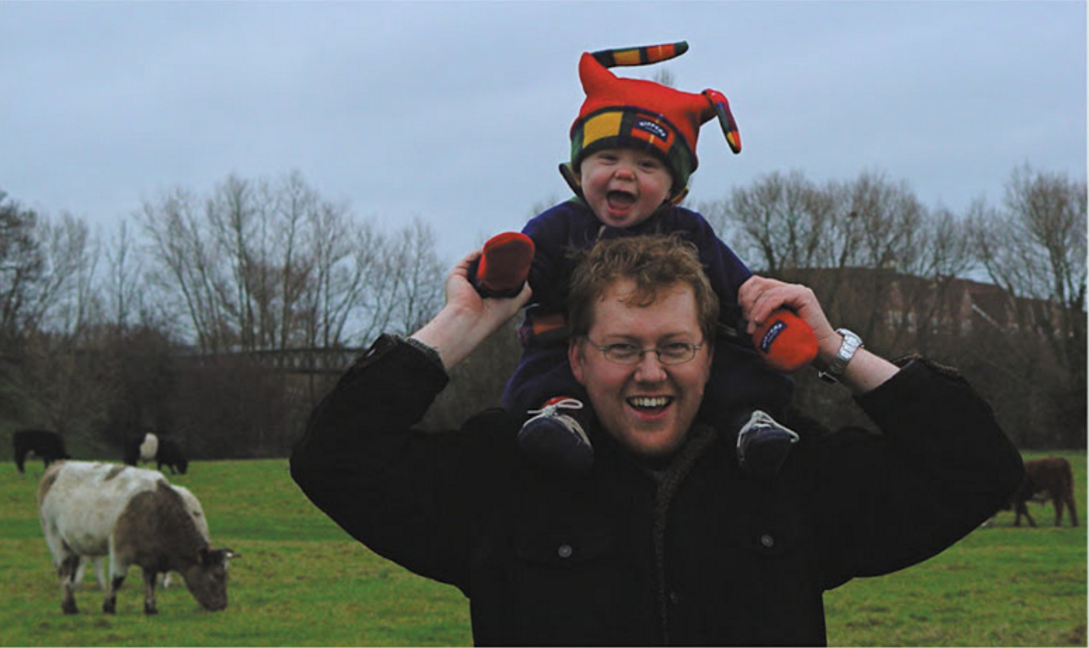
\includegraphics[width=\textwidth]{figures/rambaut.png} \\
     Andrew Rambaut \\
     UoE
     \end{figure}
\end{column}
\begin{column}{0.3\textwidth}  %%<--- here
    \begin{figure}
     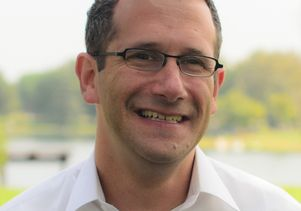
\includegraphics[width=\textwidth]{figures/suchard.png} \\
     Marc Suchard \\
     UCLA
     \end{figure}
\end{column}
\begin{column}{0.3\textwidth}  %%<--- here
    \begin{figure}
     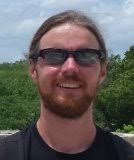
\includegraphics[width=\textwidth]{figures/baele.png} \\
     Guy Baele \\
     KU Leuven
     \end{figure}
\end{column}
\end{columns}
\end{frame}

%-=-=-=-=-=-=-=-=-=-=-=-=-=-=-=-=-=-=-=-=-=-=-=-=
%	FRAME: Motivation
%-=-=-=-=-=-=-=-=-=-=-=-=-=-=-=-=-=-=-=-=-=-=-=-=
\begingroup
% \setbeamercolor{frametitle}{bg=\cnRed}
% \setbeamercolor{normal text}{fg=\cnDarkGrey,bg=\cnLightRed}
\begin{frame}{Motivation}
\begin{block}{Phylodynamics of fast-evolving viruses}
 Inferring spatial and temporal dynamics from genomic data:
 \begin{center}
  \Large \textbf{Phylogenies}$^\ast$! \\
  \tiny $^\ast$ plus complicated models
 \end{center}
\end{block}
\begin{figure}
	\centerline{
	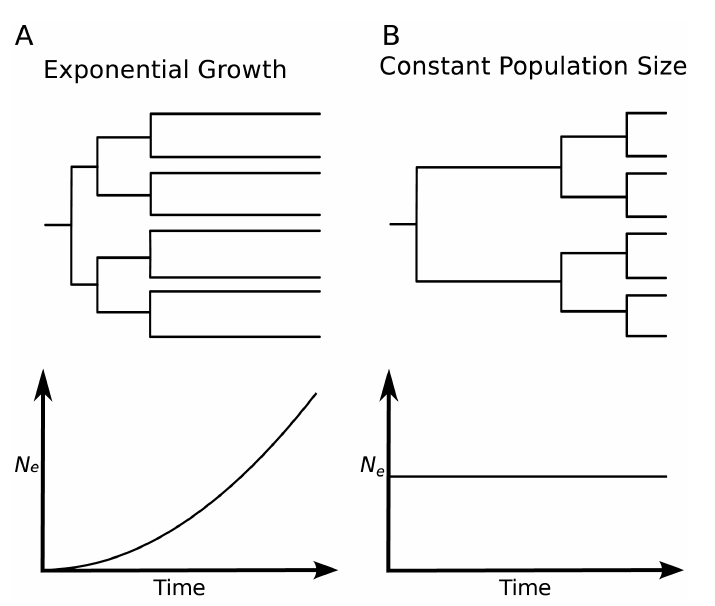
\includegraphics[width=0.5\textwidth,height=5cm]{figures/pop_growth.jpg} \\ 
	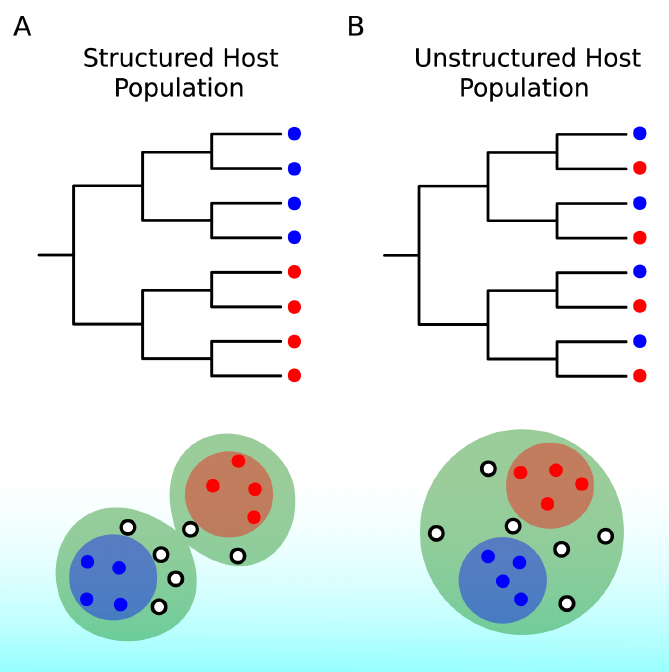
\includegraphics[width=0.5\textwidth,height=5cm]{figures/pop_structure.jpg}
	}
\end{figure}
\end{frame}
\endgroup

%-=-=-=-=-=-=-=-=-=-=-=-=-=-=-=-=-=-=-=-=-=-=-=-=
%	FRAME: estimating trees
%-=-=-=-=-=-=-=-=-=-=-=-=-=-=-=-=-=-=-=-=-=-=-=-=
\begin{frame}{Trees are hypotheses}
\begin{figure}
	\centerline{
	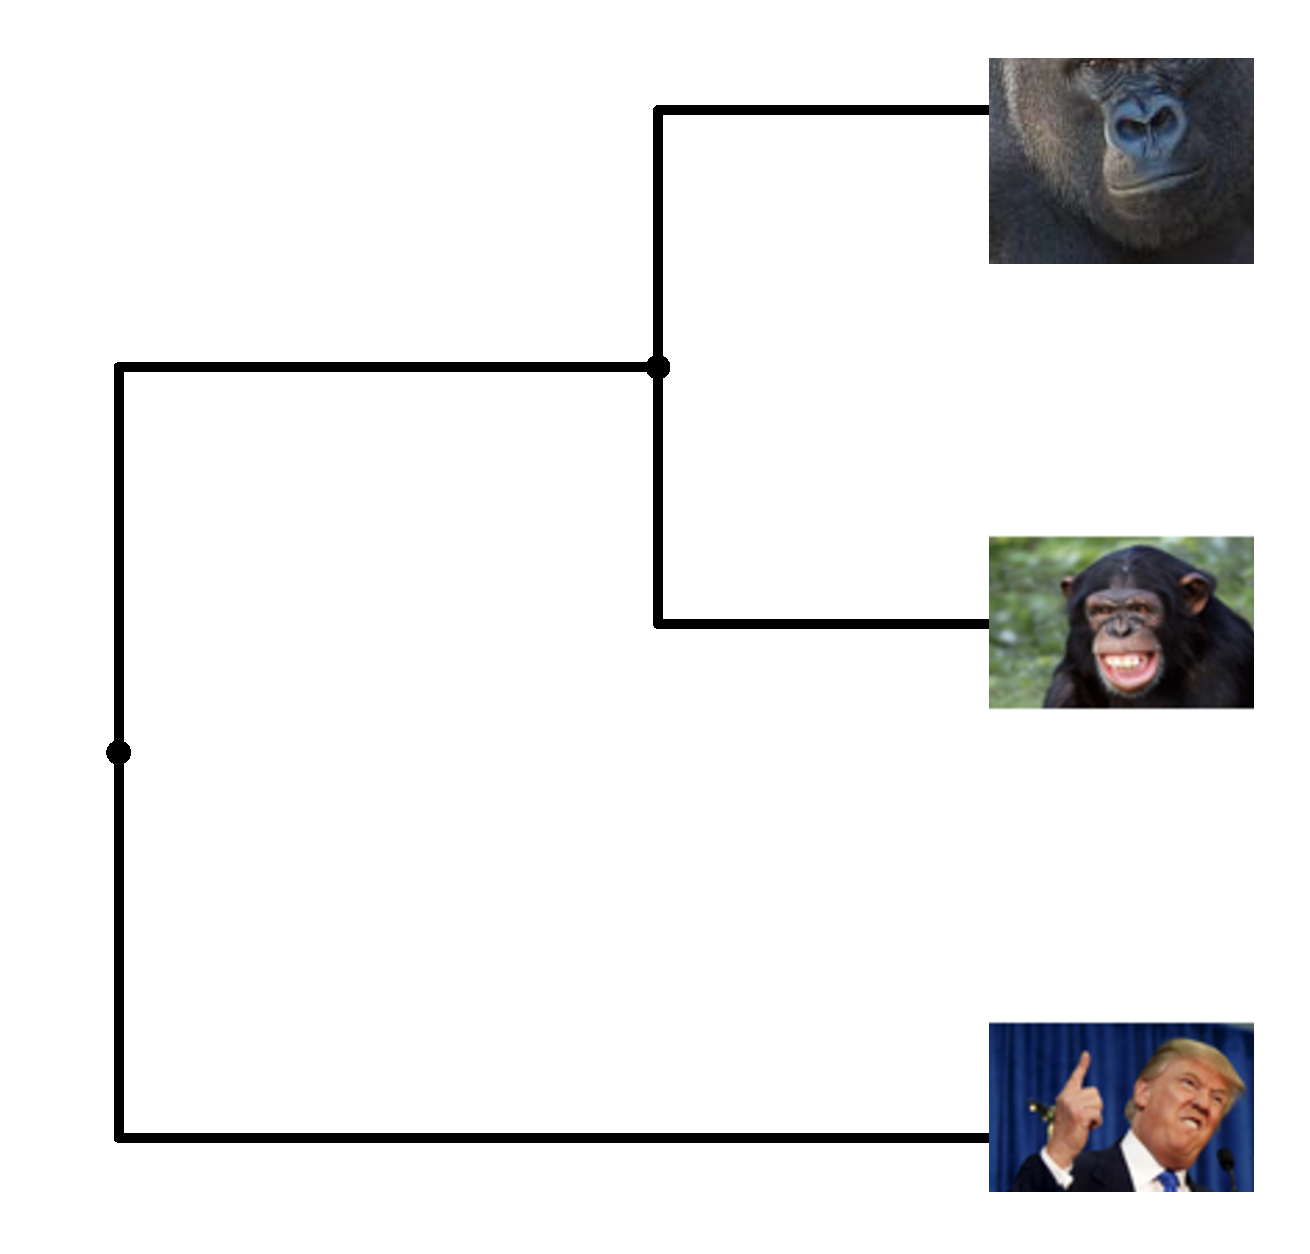
\includegraphics[width=0.3\textwidth,height=5cm]{figures/primate_tree_wrong1.pdf} \\ 
	\hspace{3em}
	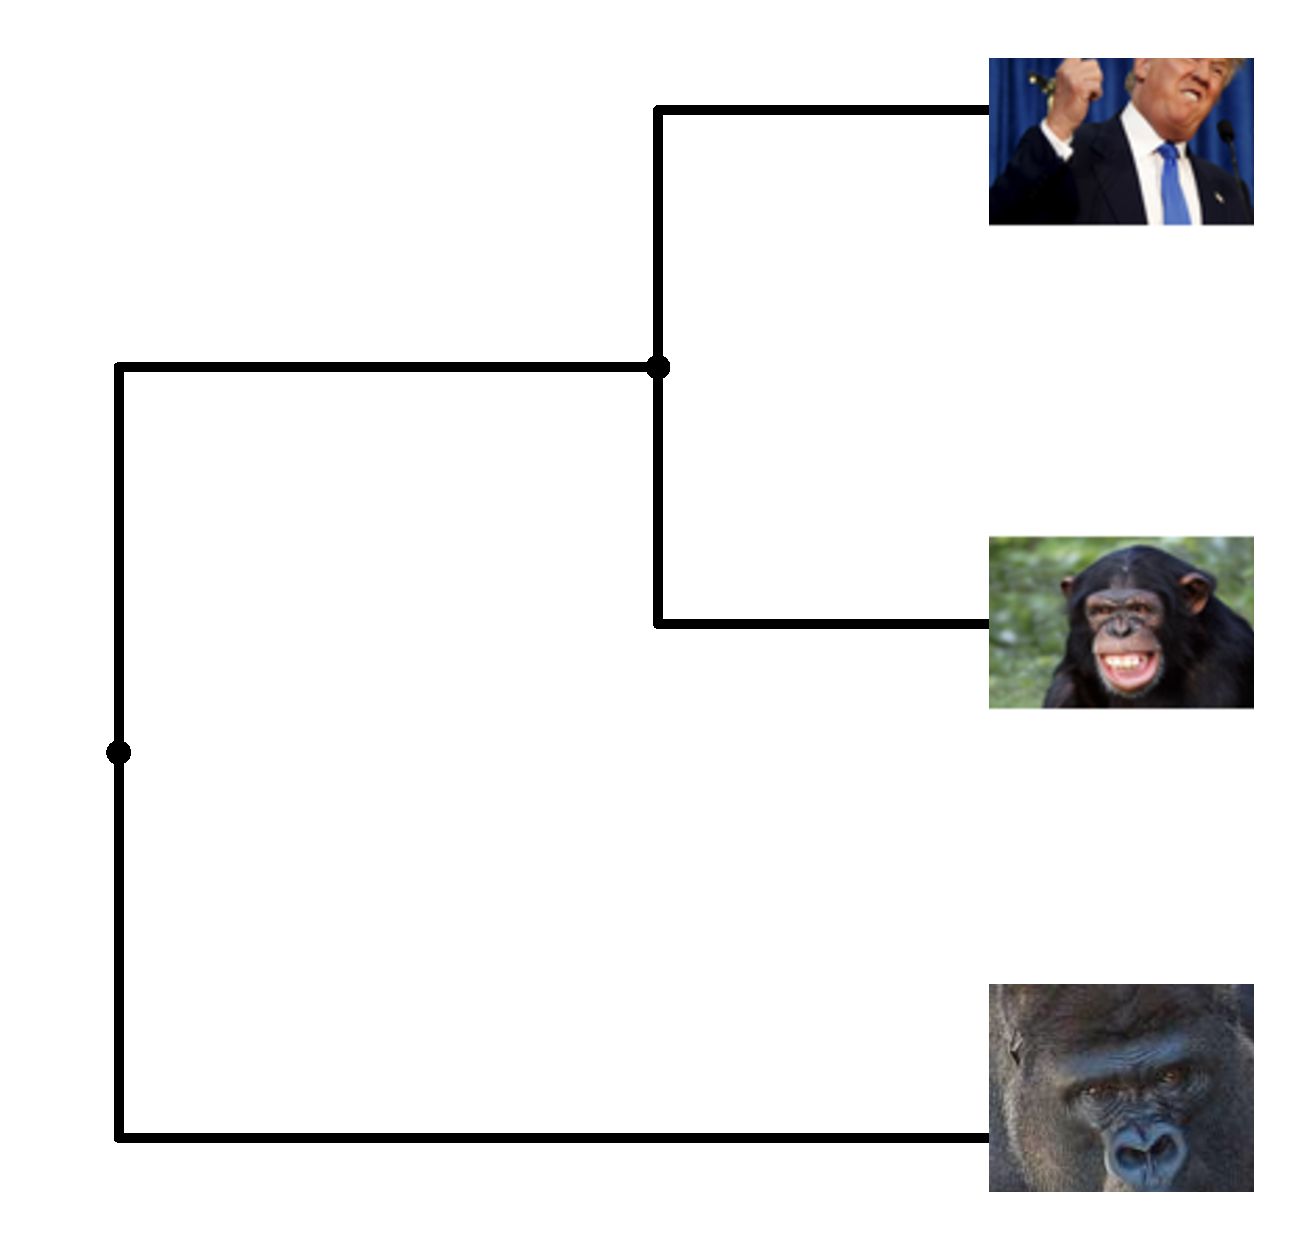
\includegraphics[width=0.3\textwidth,height=5cm]{figures/primate_tree_correct.pdf}\\
	\hspace{3em}
	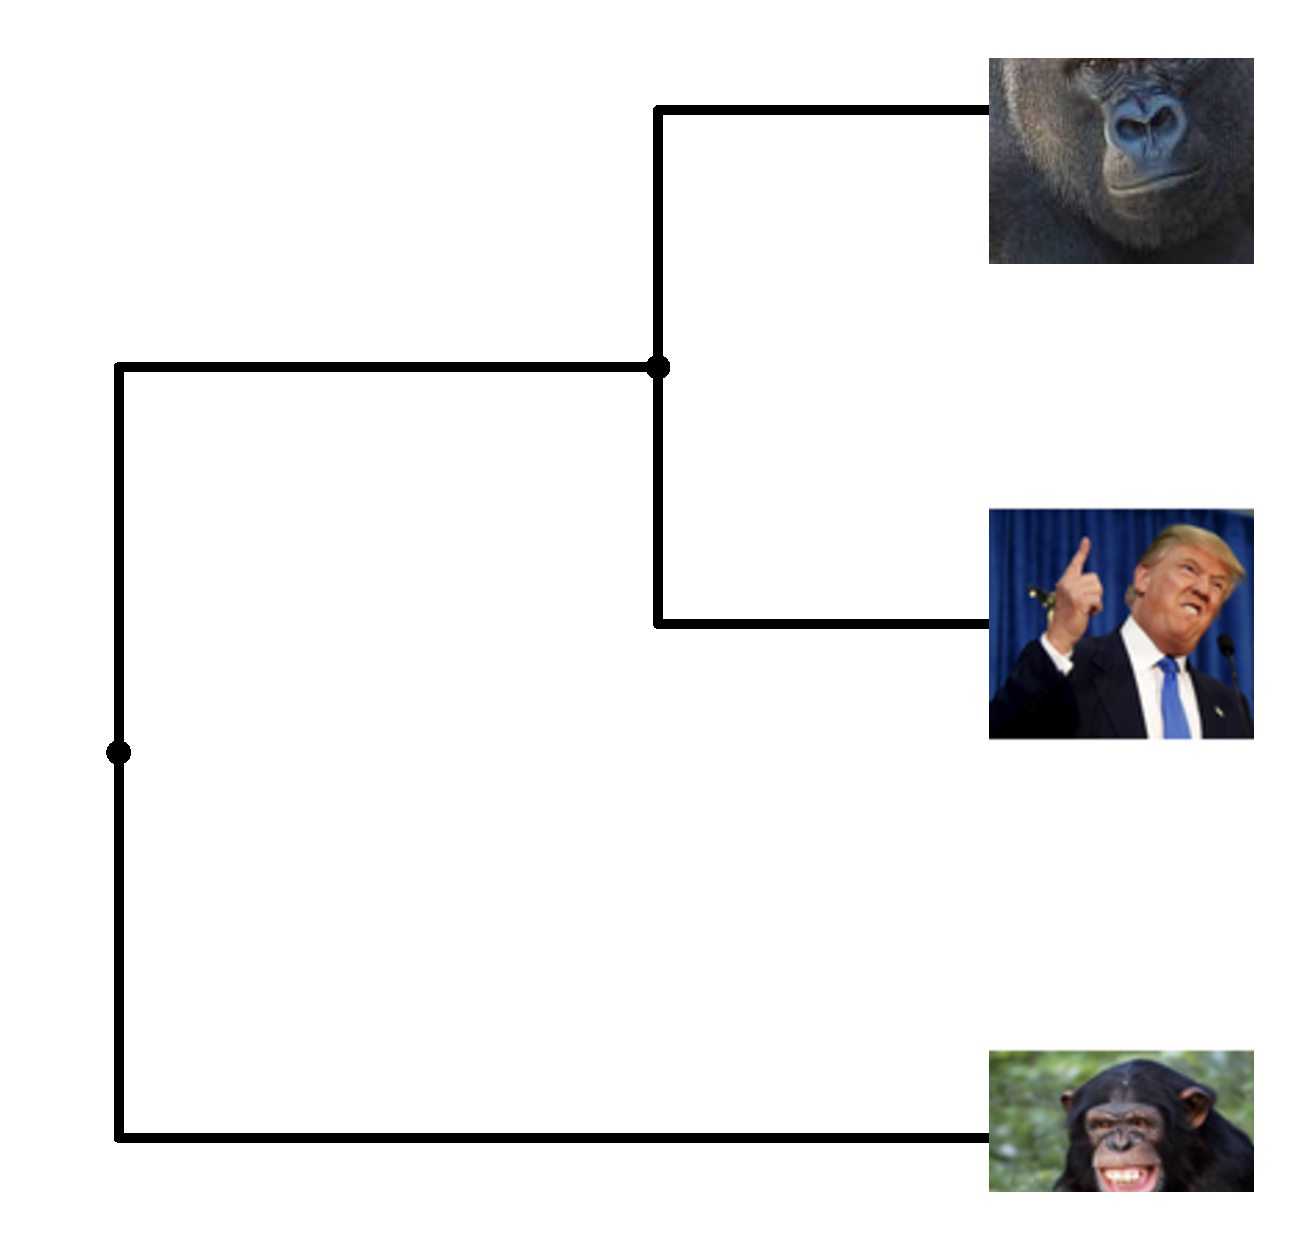
\includegraphics[width=0.3\textwidth,height=5cm]{figures/primate_tree_wrong2.pdf}
	}
\end{figure}
\end{frame}

%-=-=-=-=-=-=-=-=-=-=-=-=-=-=-=-=-=-=-=-=-=-=-=-=
%	FRAME: gist of BP
%-=-=-=-=-=-=-=-=-=-=-=-=-=-=-=-=-=-=-=-=-=-=-=-=
\begin{frame}{The gist of Bayesian phylogenetics}
\begin{block}{Bayesian paradigm:}
 \textbf{Marginalise} (integrate), not maximise
\end{block}
\vspace{2em}
\begin{figure}
	\centerline{
	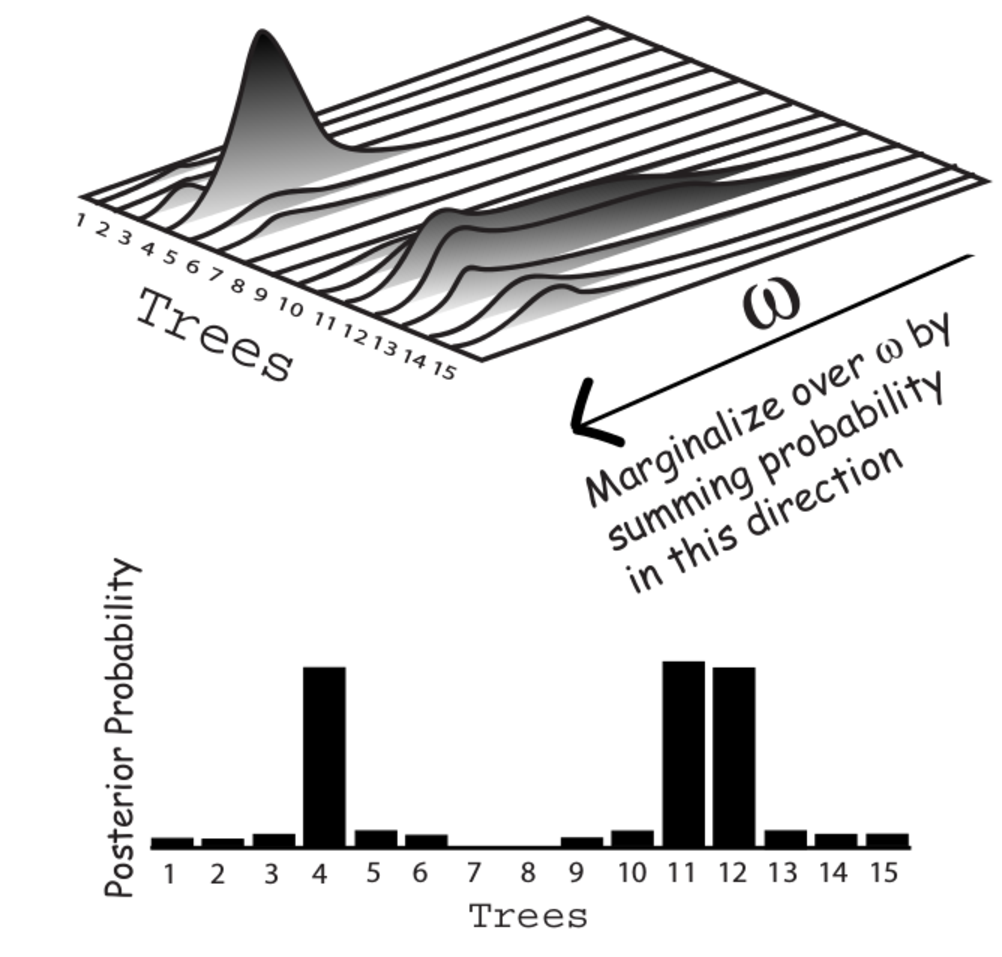
\includegraphics[width=0.55\textwidth,height=6cm]{figures/Joint_trees_omega_marg1.pdf} \\ 
	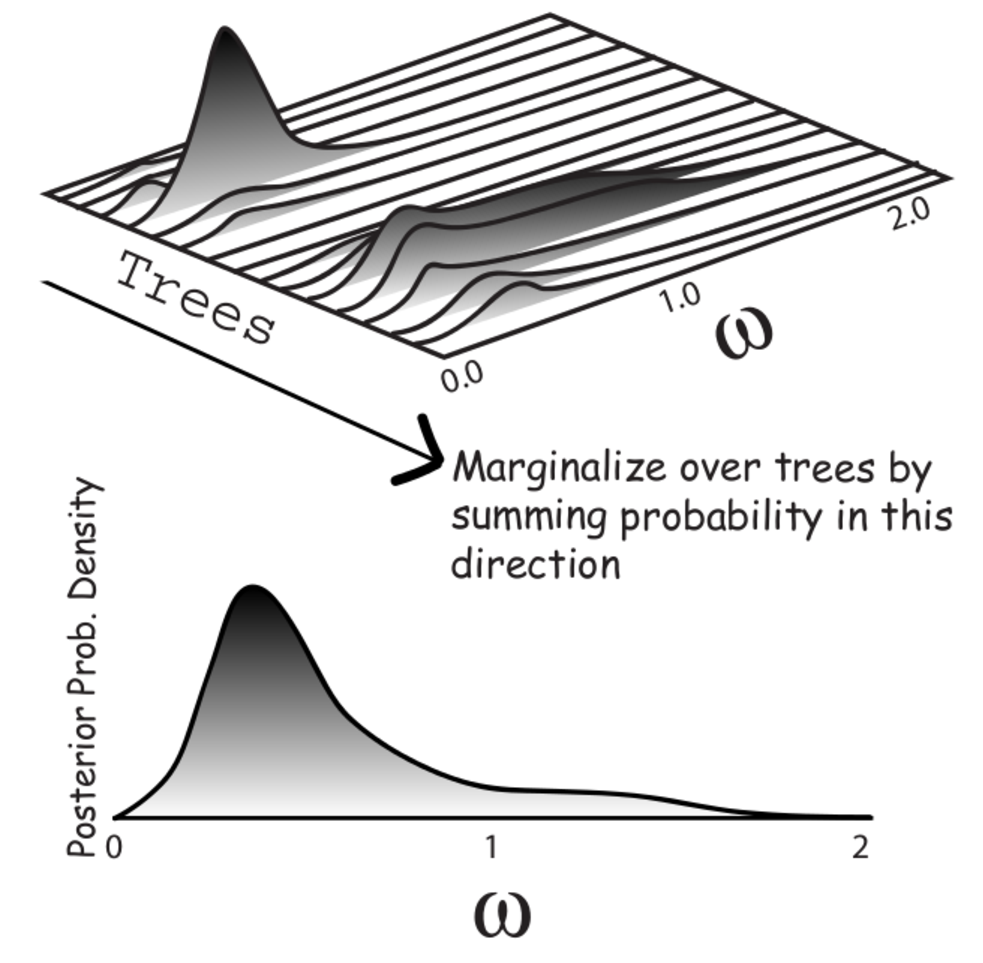
\includegraphics[width=0.55\textwidth,height=6cm]{figures/Joint_trees_omega_marg2.pdf}
	}
\end{figure}
\end{frame}

%-=-=-=-=-=-=-=-=-=-=-=-=-=-=-=-=-=-=-=-=-=-=-=-=
%	FRAME: Tree space
%-=-=-=-=-=-=-=-=-=-=-=-=-=-=-=-=-=-=-=-=-=-=-=-=
\begin{frame}{Tree space: a strange land}
 \begin{column}{0.55\textwidth}
\begin{figure}
	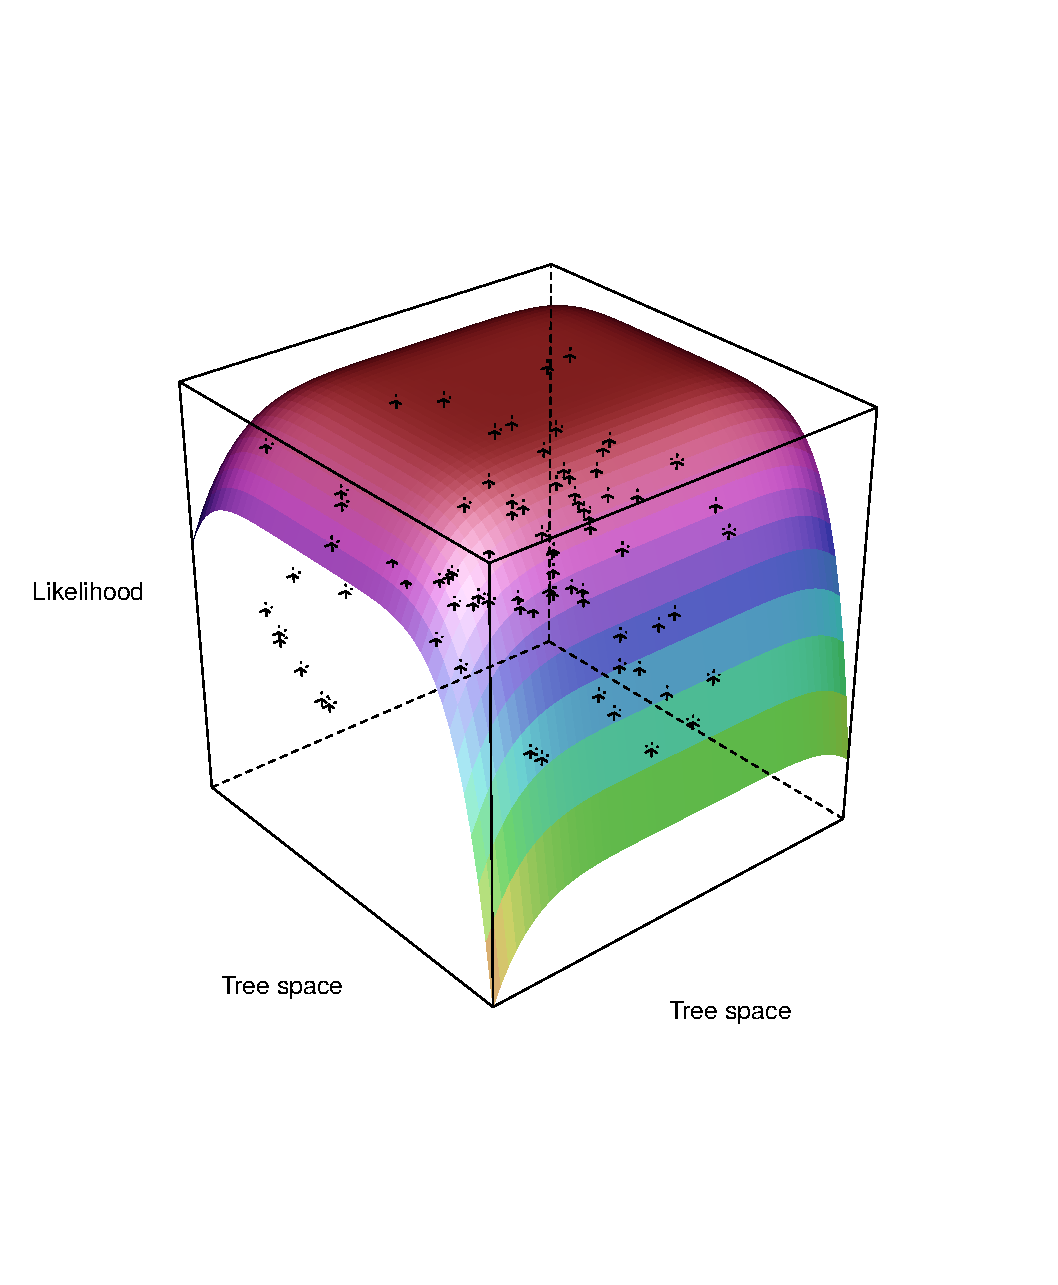
\includegraphics[width=\textwidth,height=8cm]{figures/treespace_5taxa_likelihood.pdf}
\end{figure}
\end{column}
 \begin{column}{0.45\textwidth}
\begin{figure}
	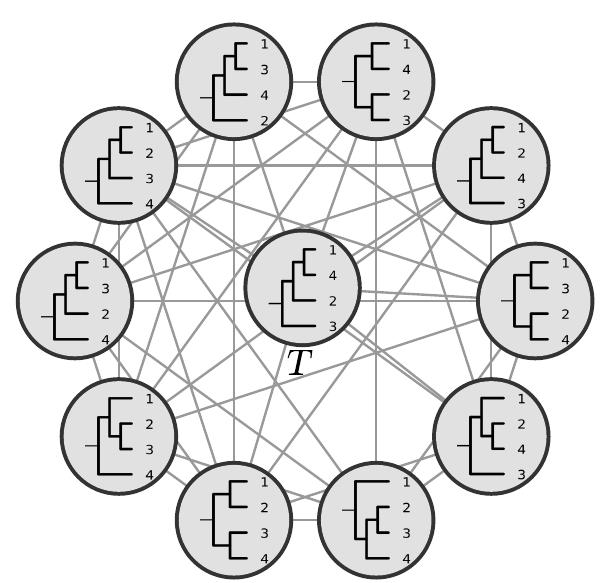
\includegraphics[width=\textwidth,height=6cm]{figures/spr_graph.jpg}
\end{figure}
\end{column}
\end{frame}

%-=-=-=-=-=-=-=-=-=-=-=-=-=-=-=-=-=-=-=-=-=-=-=-=
%	FRAME: Metropolis-Hastings
%-=-=-=-=-=-=-=-=-=-=-=-=-=-=-=-=-=-=-=-=-=-=-=-=
\begin{frame}{Metropolis-Hastings algorithm}
\begin{figure}
	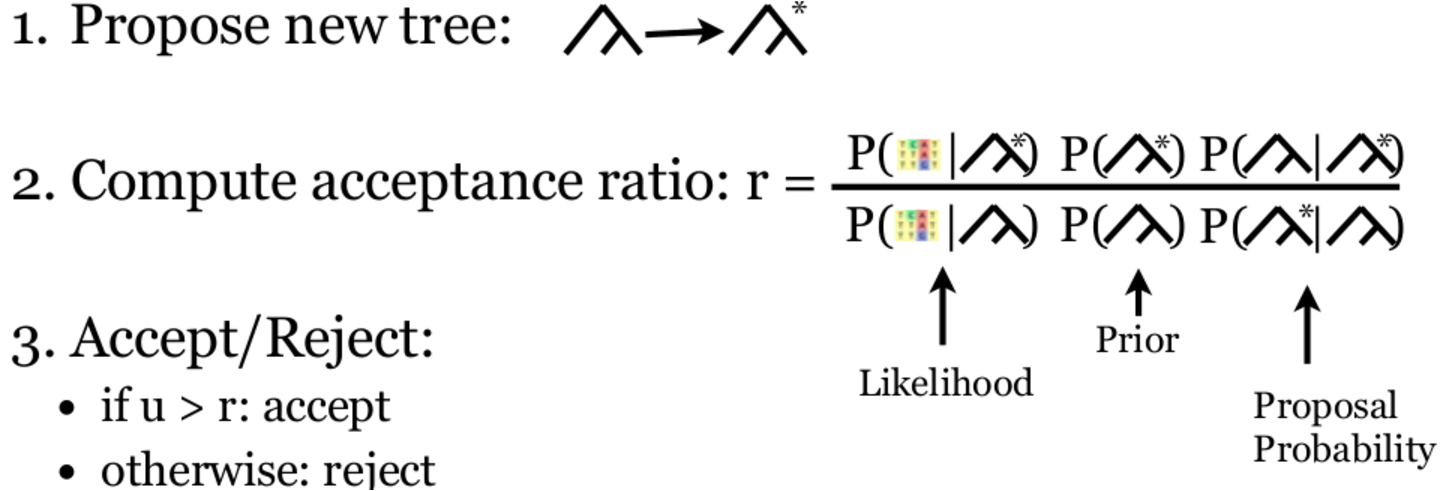
\includegraphics[width=0.85\textwidth,height=4.5cm]{figures/MH.pdf} 
\end{figure}
\end{frame}

%-=-=-=-=-=-=-=-=-=-=-=-=-=-=-=-=-=-=-=-=-=-=-=-=
%	FRAME:Robot
%-=-=-=-=-=-=-=-=-=-=-=-=-=-=-=-=-=-=-=-=-=-=-=-=
\begin{frame}{MCMC ``robot''}
\begin{figure}
	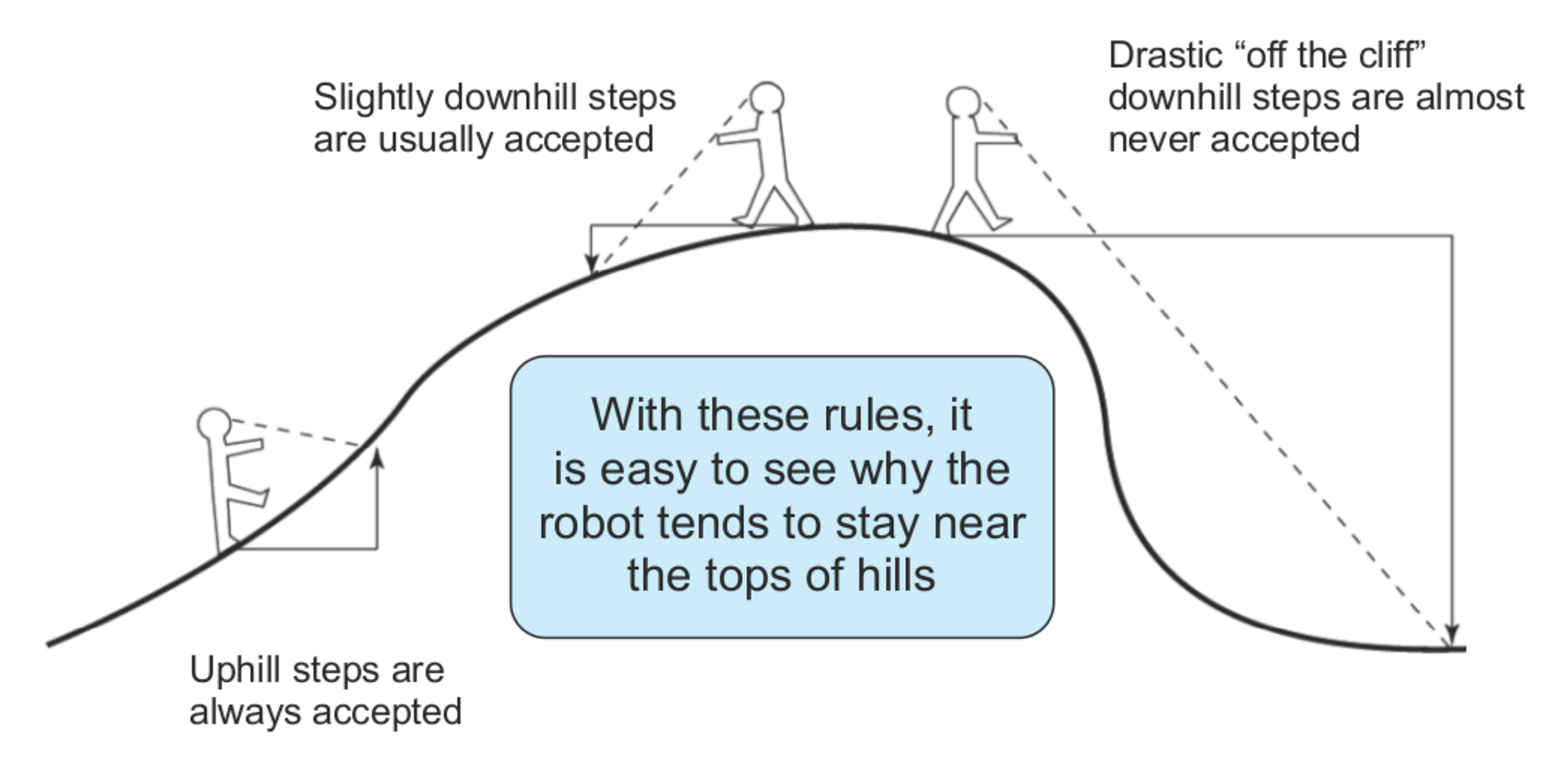
\includegraphics[width=0.85\textwidth,height=6cm]{figures/robot.pdf} 
\end{figure}
\end{frame}

%-=-=-=-=-=-=-=-=-=-=-=-=-=-=-=-=-=-=-=-=-=-=-=-=
%	FRAME: Exploring parameter space I
%-=-=-=-=-=-=-=-=-=-=-=-=-=-=-=-=-=-=-=-=-=-=-=-=
\begin{frame}{Exploring parameter space: \textbf{burn-in}}
\begin{figure}
	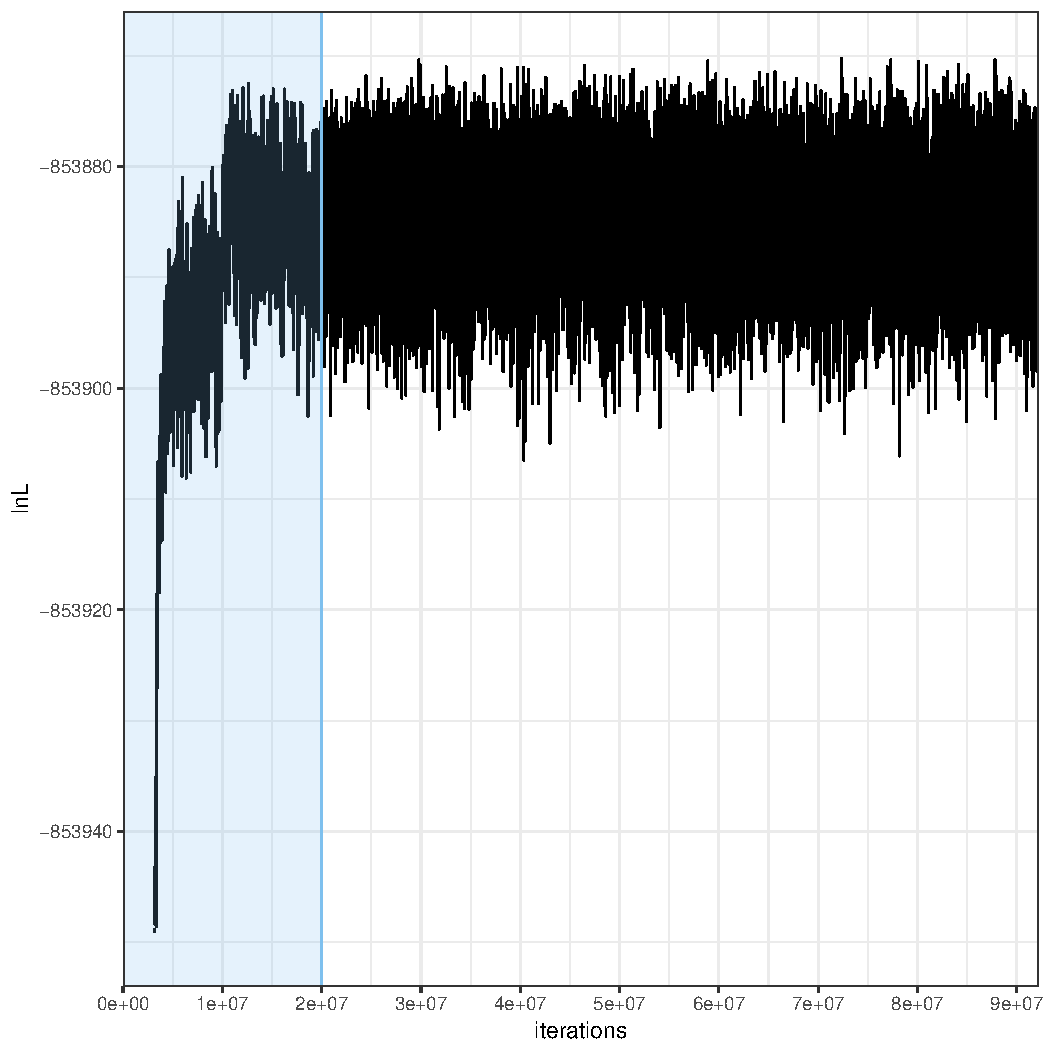
\includegraphics[width=\textwidth,height=7cm]{figures/burnin.pdf} 
\end{figure}
\end{frame}

%-=-=-=-=-=-=-=-=-=-=-=-=-=-=-=-=-=-=-=-=-=-=-=-=
%	FRAME: Exploring parameter space II
%-=-=-=-=-=-=-=-=-=-=-=-=-=-=-=-=-=-=-=-=-=-=-=-=
\begin{frame}{Exploring parameter space: \textbf{mixing}}
\begin{figure}
	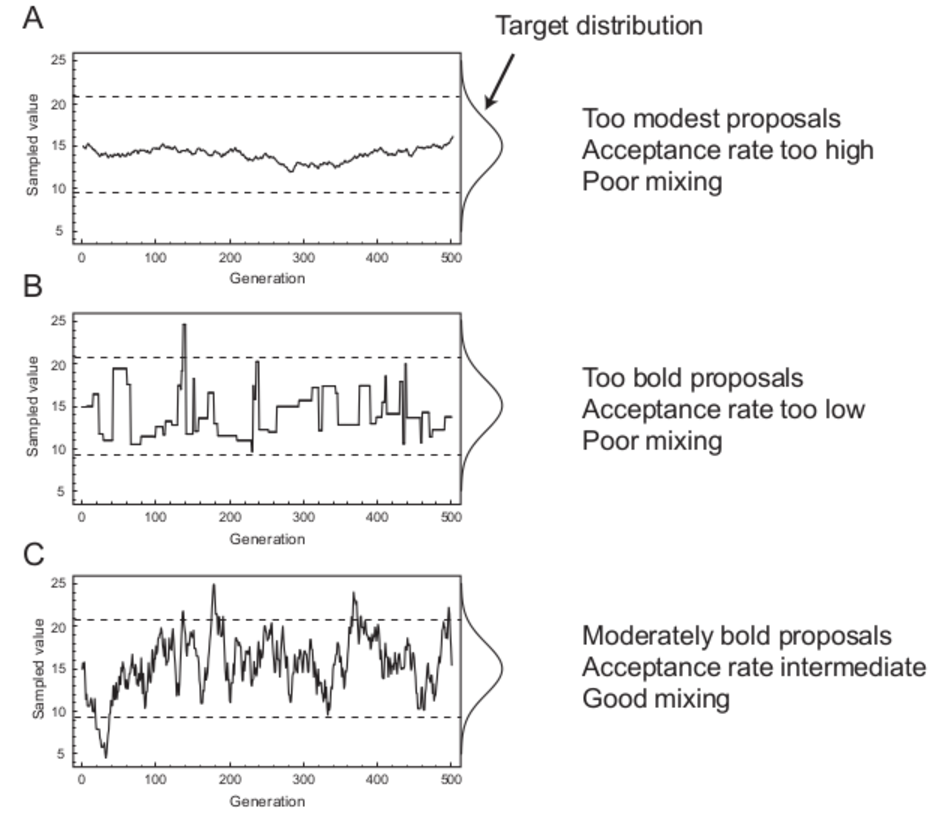
\includegraphics[width=\textwidth,height=8cm]{figures/mixing.pdf} 
\end{figure}
\end{frame}

%-=-=-=-=-=-=-=-=-=-=-=-=-=-=-=-=-=-=-=-=-=-=-=-=
%	FRAME: Time-tree kernels
%-=-=-=-=-=-=-=-=-=-=-=-=-=-=-=-=-=-=-=-=-=-=-=-=
\begin{frame}{Height-preserving kernels: SubTreeLeap}
\begin{figure}
	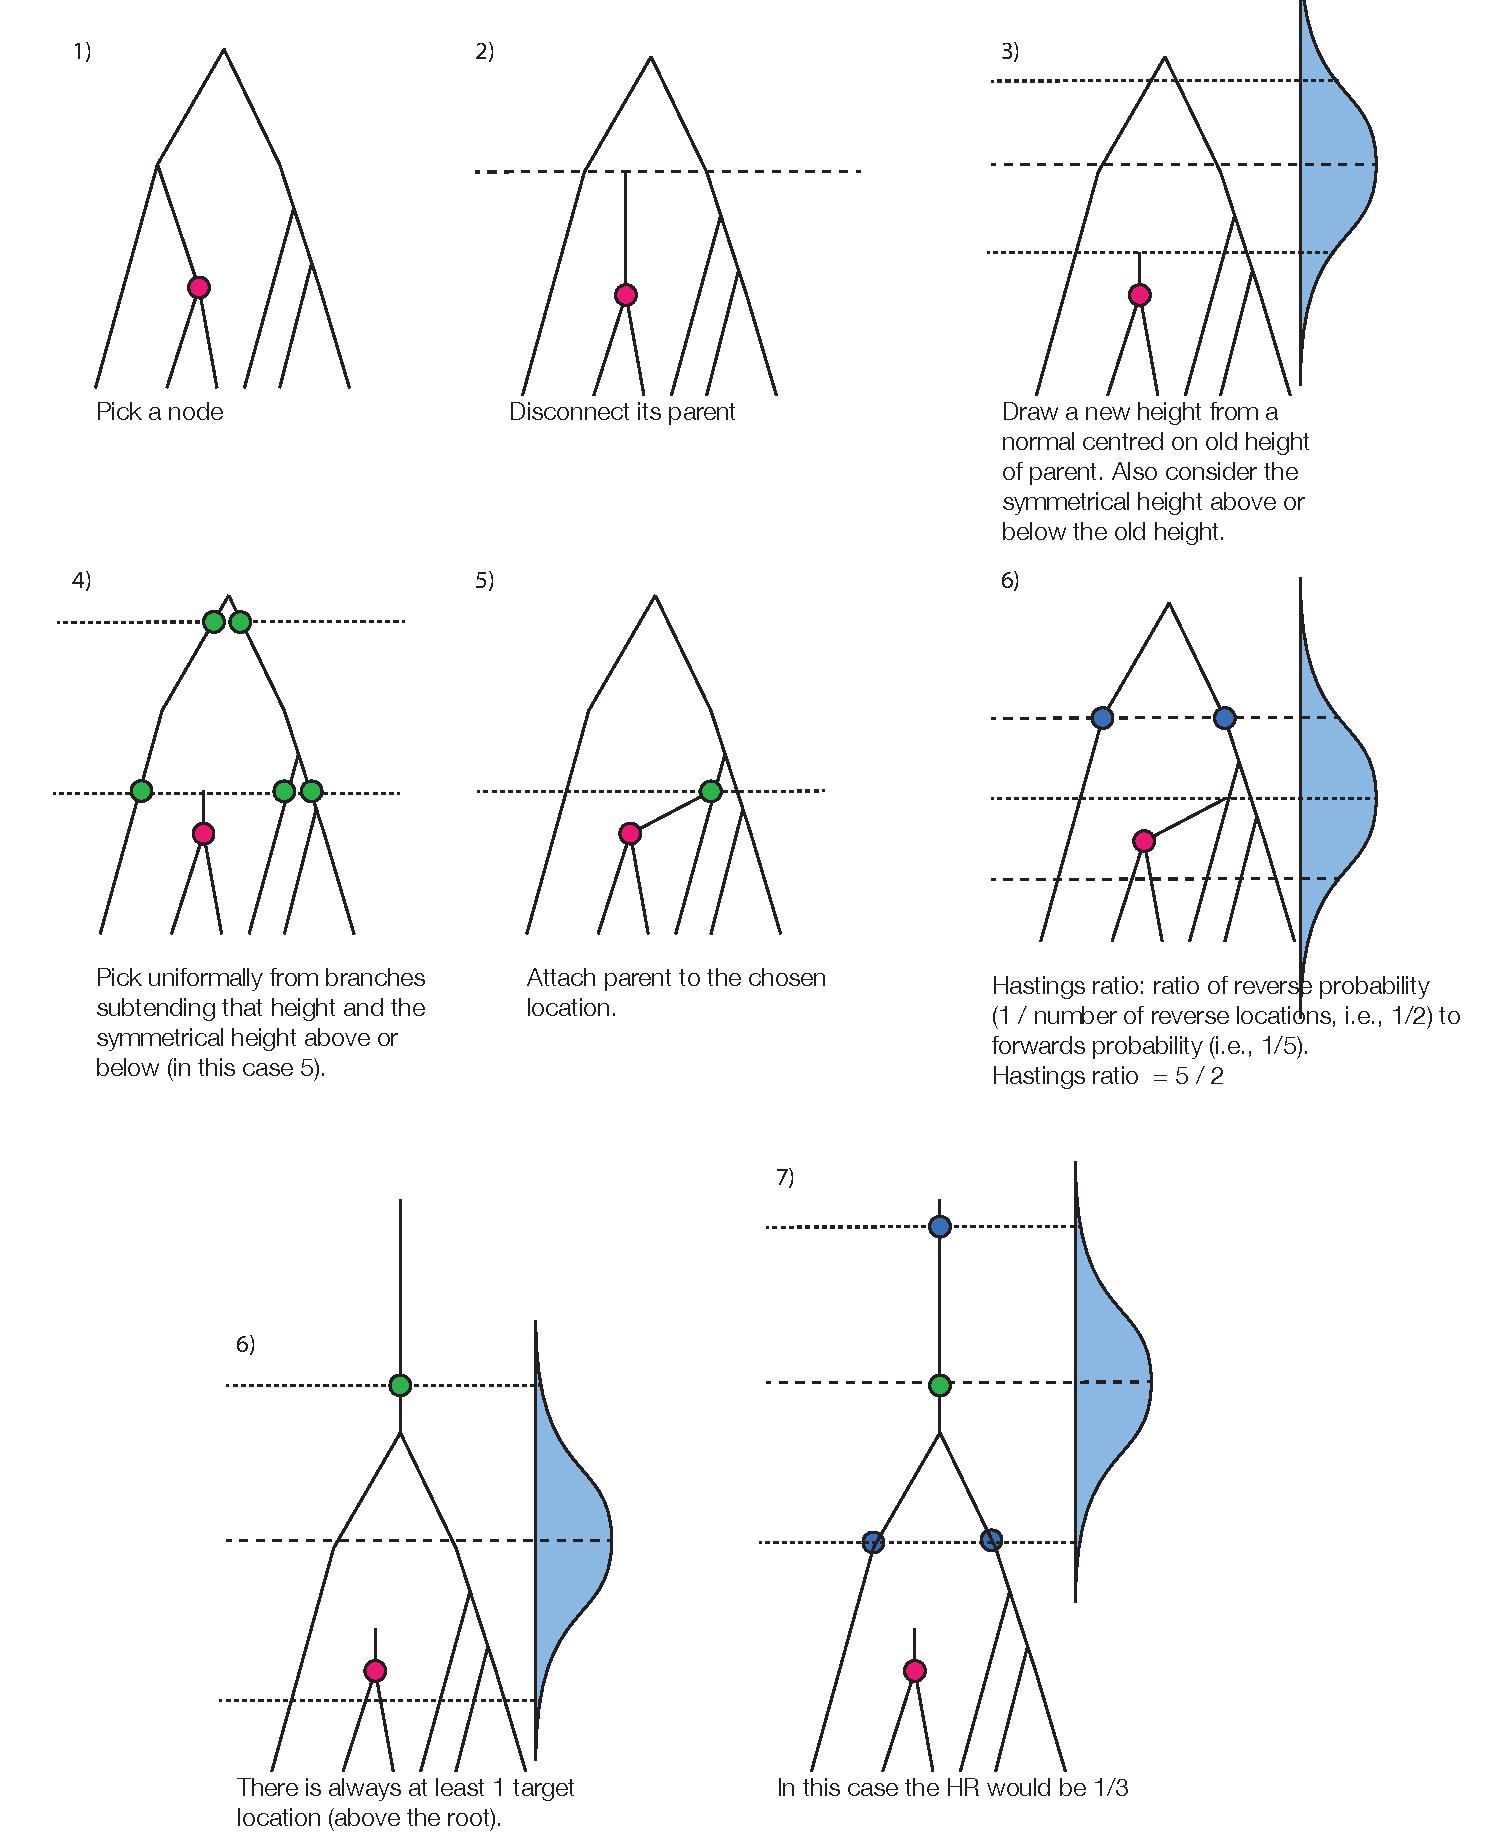
\includegraphics[width=\textwidth,height=8cm]{figures/STL_kernel.pdf} 
\end{figure}
\end{frame}

%-=-=-=-=-=-=-=-=-=-=-=-=-=-=-=-=-=-=-=-=-=-=-=-=
%	FRAME: Results Denv4
%-=-=-=-=-=-=-=-=-=-=-=-=-=-=-=-=-=-=-=-=-=-=-=-=
\begin{frame}{Dengue 4 \textit{env} (17 taxa, 1485 sites)}
\begin{figure}
\begin{column}{0.5\textwidth}
    \begin{figure}
     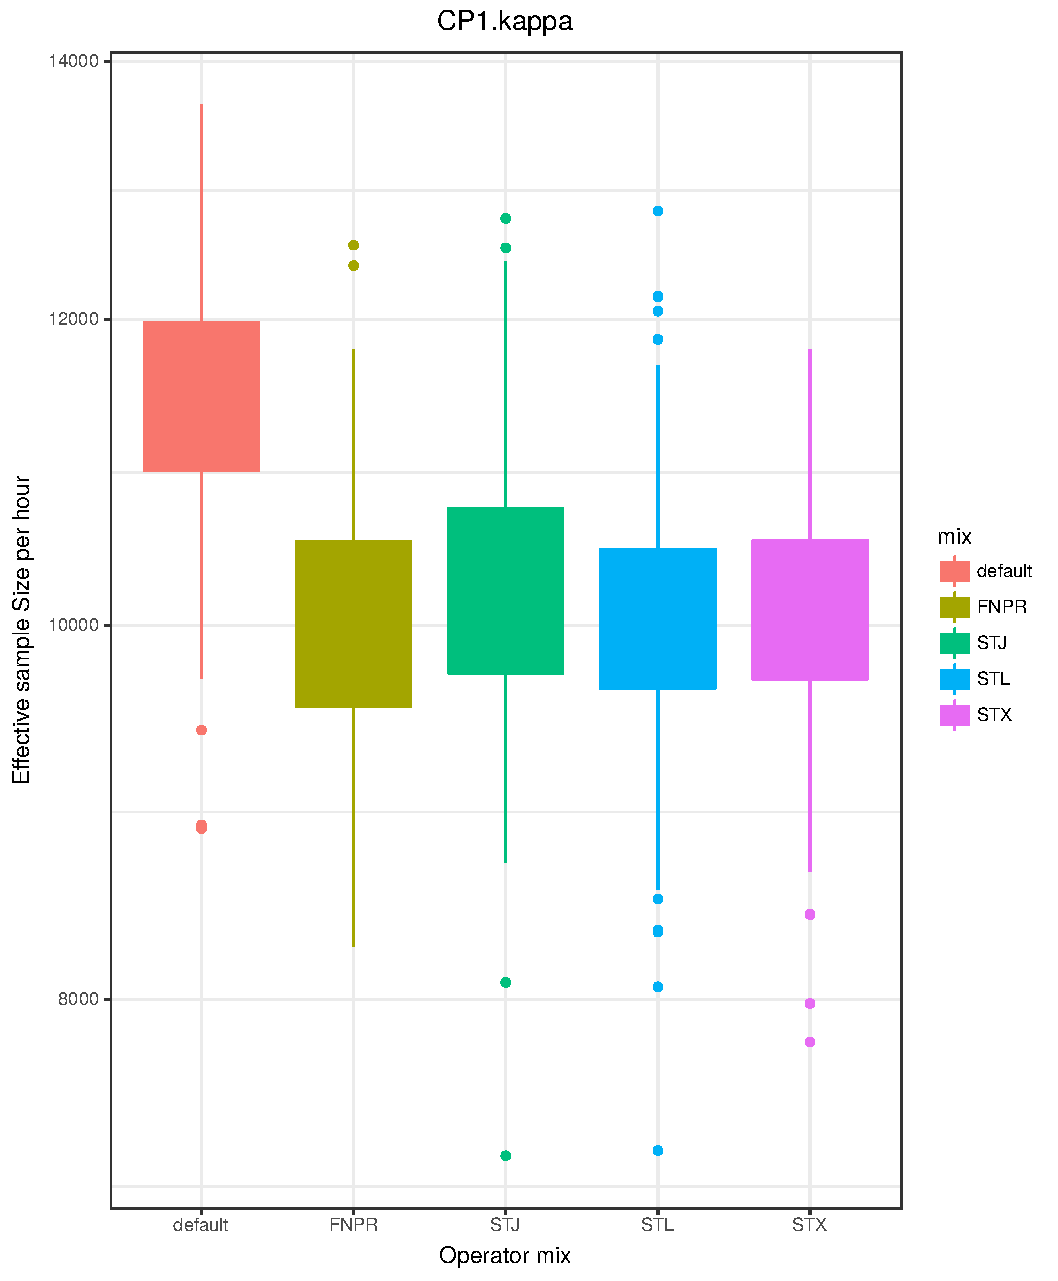
\includegraphics[width=\textwidth]{figures/ESS_hour_CP1Kappa_dengue4.pdf} \\
     \end{figure}
\end{column}
\begin{column}{0.5\textwidth}  %%<--- here
    \begin{figure}
     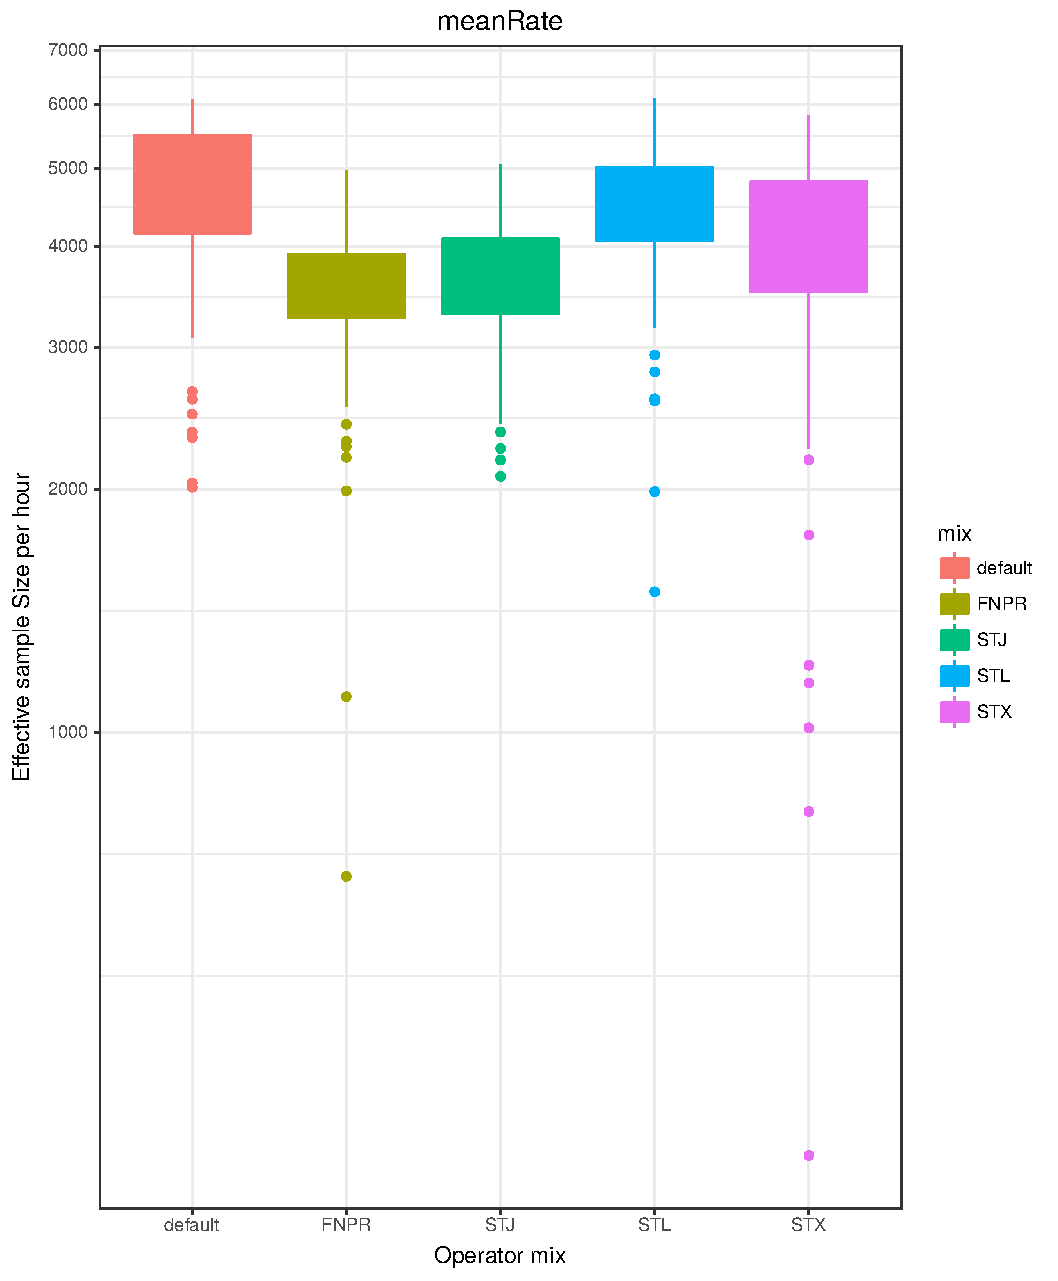
\includegraphics[width=\textwidth]{figures/ESS_hour_meanRate_dengue4.pdf} \\
     \end{figure}
\end{column}
\end{figure}
\end{frame}

%-=-=-=-=-=-=-=-=-=-=-=-=-=-=-=-=-=-=-=-=-=-=-=-=
%	FRAME: Results RSVA
%-=-=-=-=-=-=-=-=-=-=-=-=-=-=-=-=-=-=-=-=-=-=-=-=
\begin{frame}{RSVA G protein (35 taxa, 629 sites)}
\begin{figure}
\begin{column}{0.5\textwidth}
    \begin{figure}
     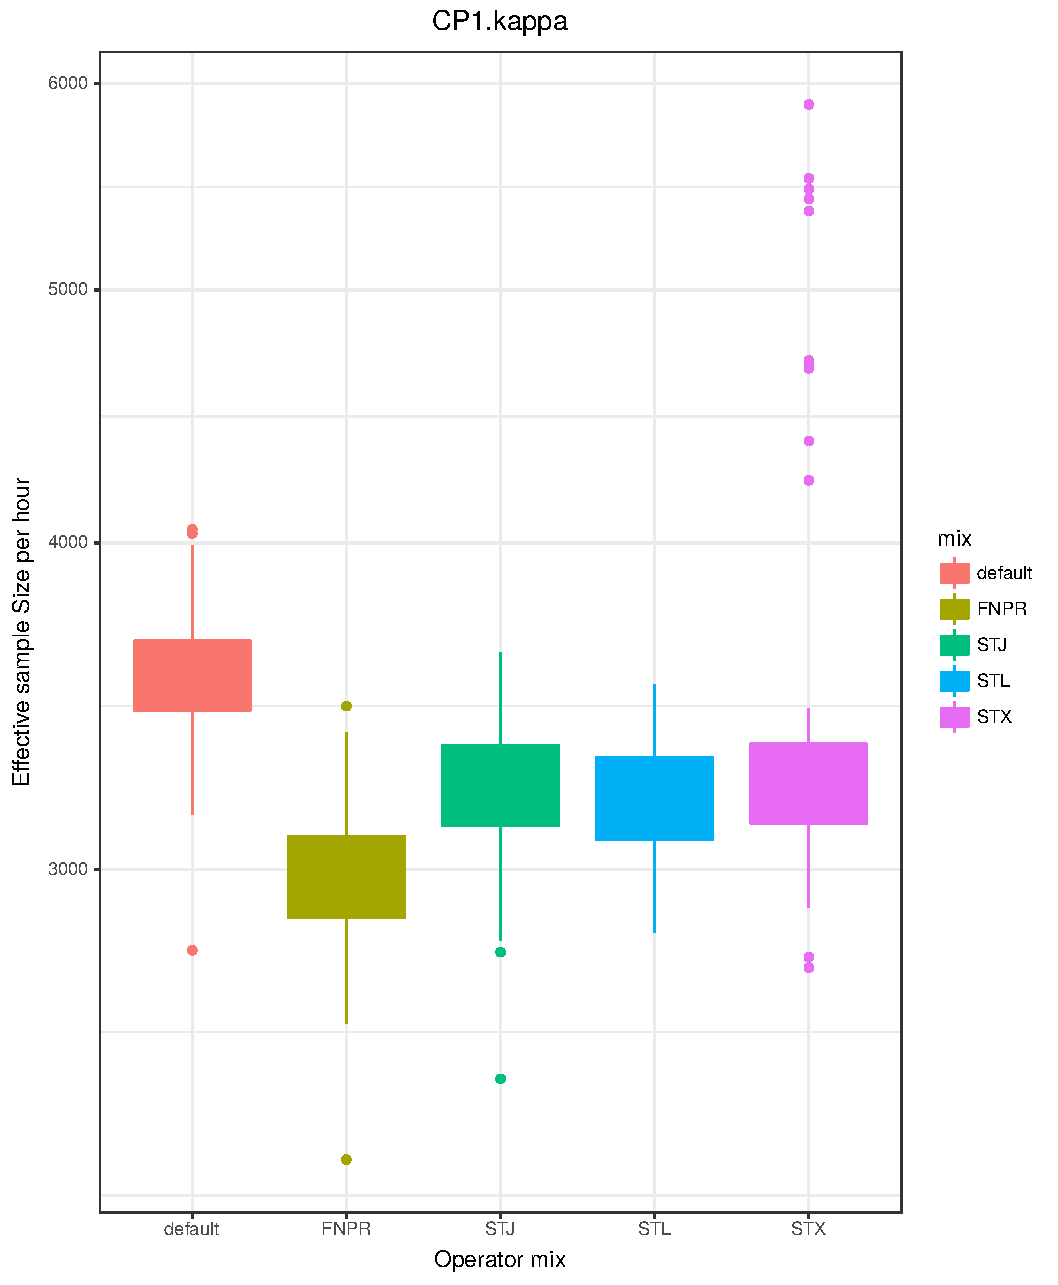
\includegraphics[width=\textwidth]{figures/ESS_hour_CP1Kappa_RSVA.pdf} \\
     \end{figure}
\end{column}
\begin{column}{0.5\textwidth}  %%<--- here
    \begin{figure}
     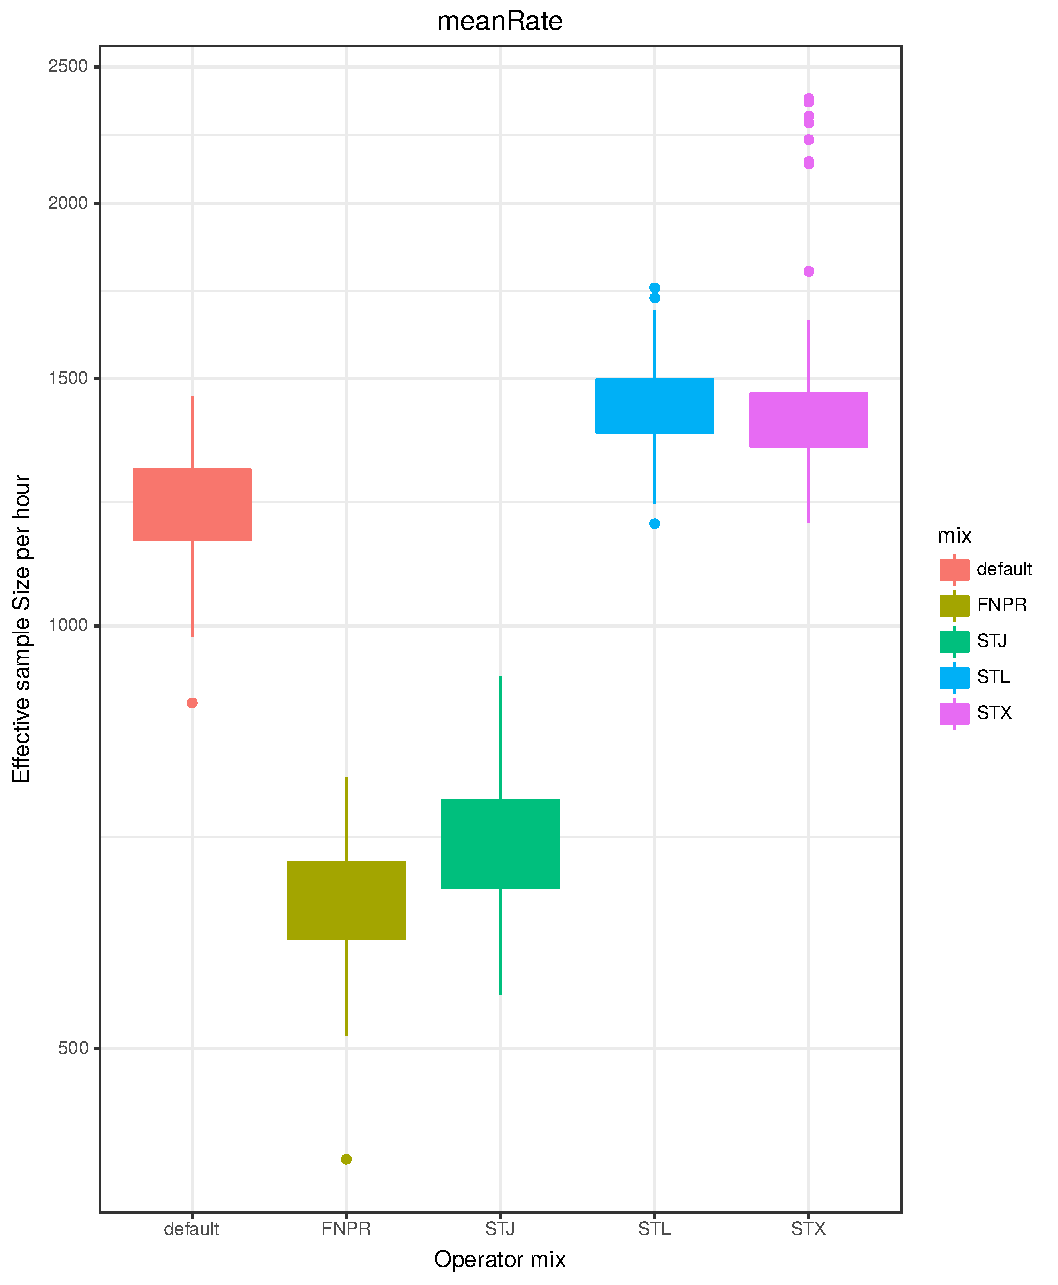
\includegraphics[width=\textwidth]{figures/ESS_hour_meanRate_RSVA.pdf} \\
     \end{figure}
\end{column}
\end{figure}
\end{frame}

%-=-=-=-=-=-=-=-=-=-=-=-=-=-=-=-=-=-=-=-=-=-=-=-=
%	FRAME: Results YFV
%-=-=-=-=-=-=-=-=-=-=-=-=-=-=-=-=-=-=-=-=-=-=-=-=
\begin{frame}{YFV \textit{prM/E} gene (71 taxa, 654 sites)}
\begin{figure}
\begin{column}{0.5\textwidth}
    \begin{figure}
     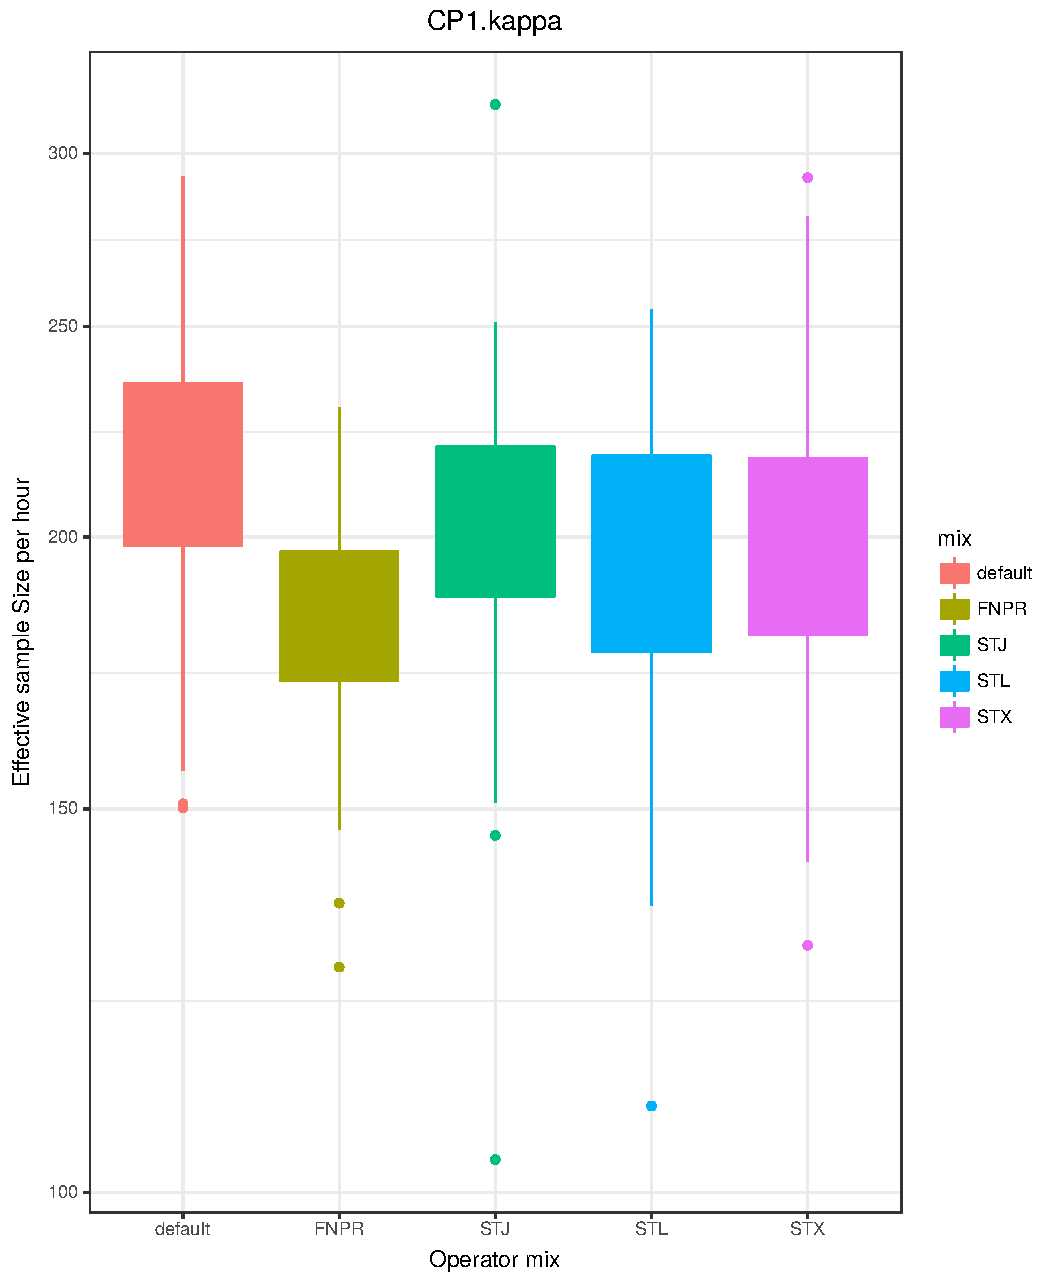
\includegraphics[width=\textwidth]{figures/ESS_hour_CP1Kappa_YFV.pdf} \\
     \end{figure}
\end{column}
\begin{column}{0.5\textwidth}  %%<--- here
    \begin{figure}
     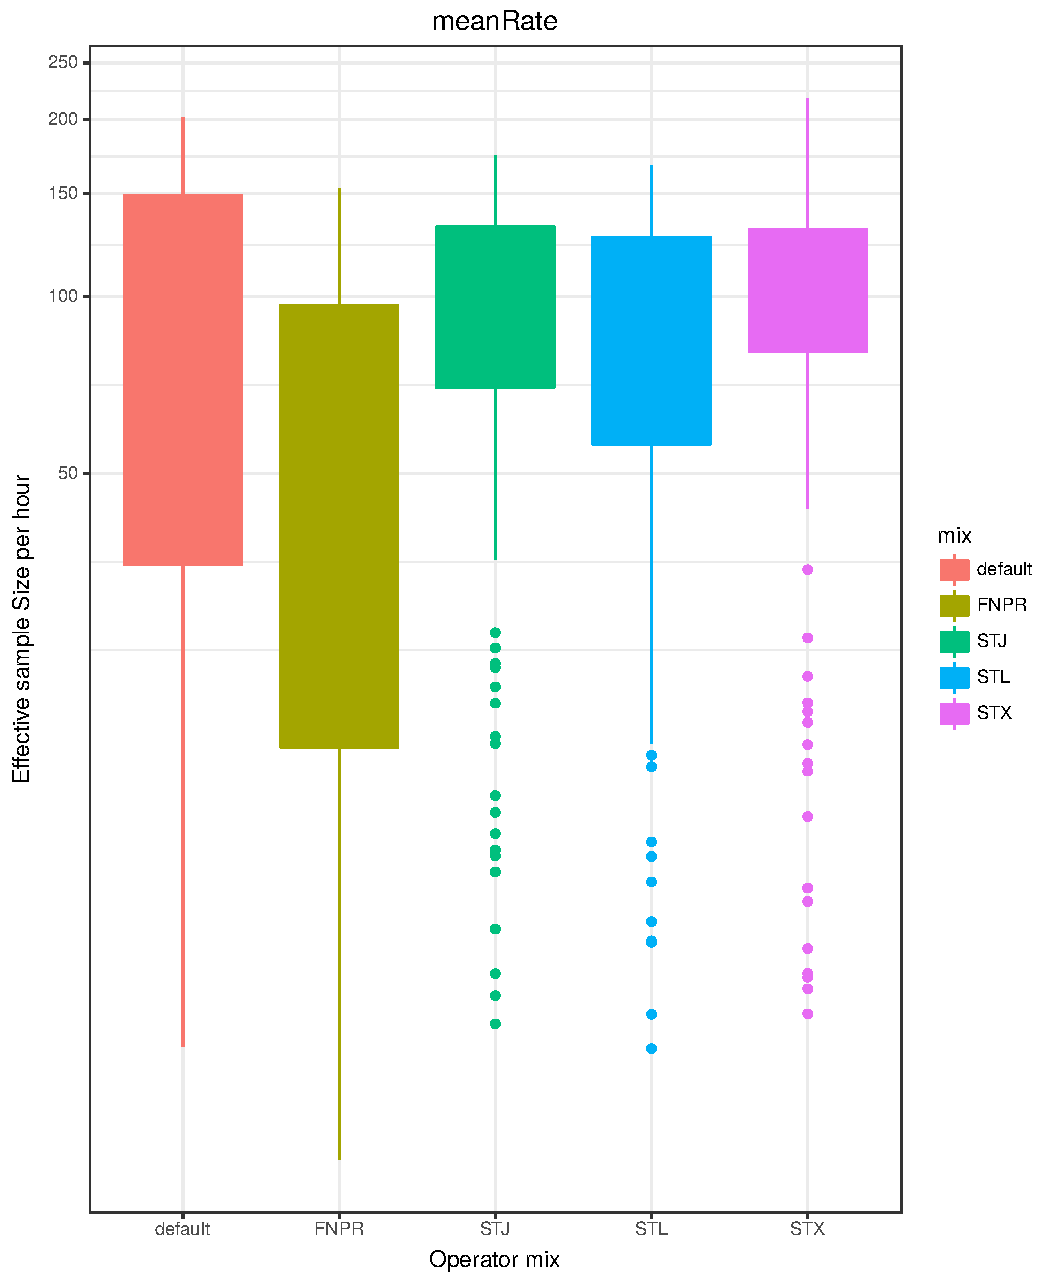
\includegraphics[width=\textwidth]{figures/ESS_hour_meanRate_YFV.pdf} \\
     \end{figure}
\end{column}
\end{figure}
\end{frame}

%-=-=-=-=-=-=-=-=-=-=-=-=-=-=-=-=-=-=-=-=-=-=-=-=
%	FRAME: Results Extra
%-=-=-=-=-=-=-=-=-=-=-=-=-=-=-=-=-=-=-=-=-=-=-=-=
\begin{frame}{Metazoans (contemporaneous, 55 taxa, 30257 AA sites)}
\begin{figure}
	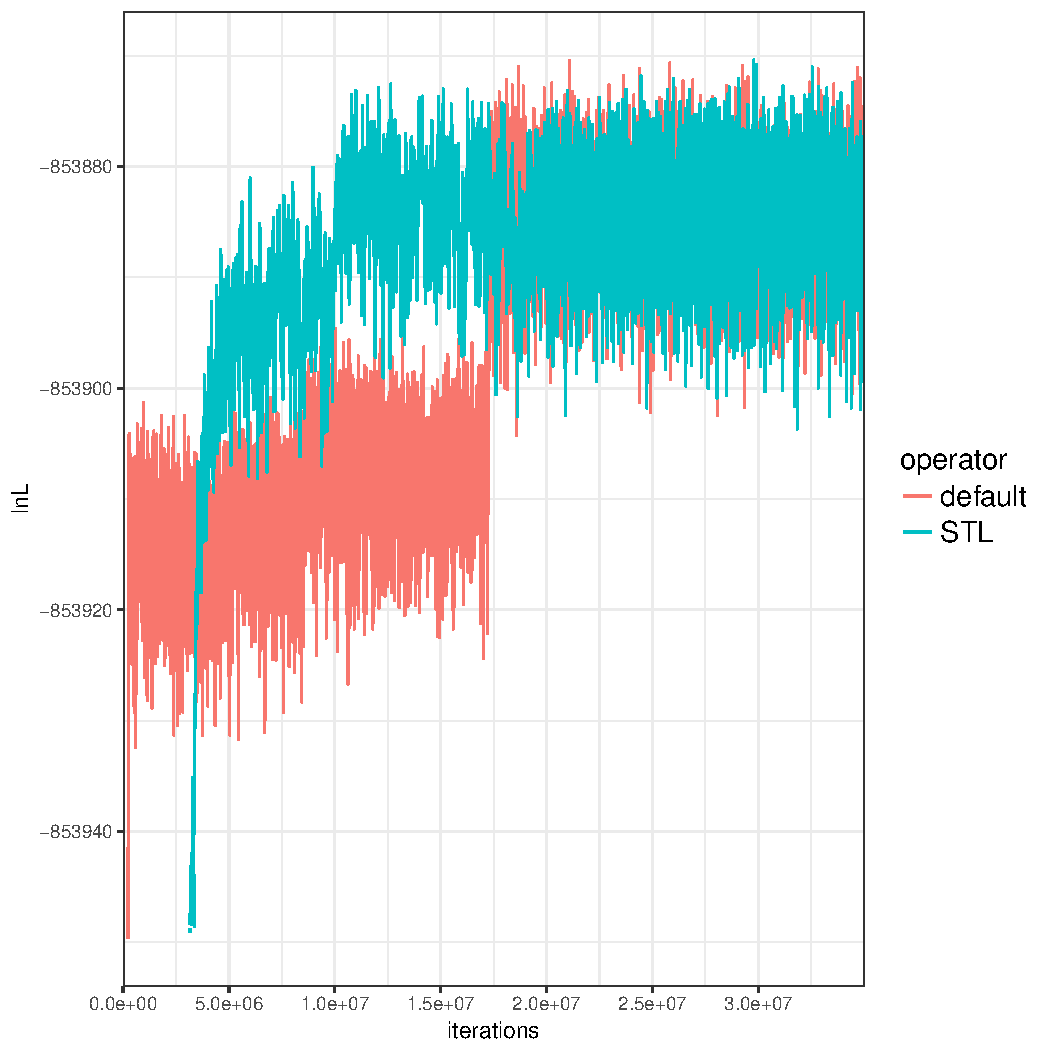
\includegraphics[width=\textwidth,height=8cm]{figures/comparison_metazoan.pdf} 
\end{figure}
\end{frame}
%-=-=-=-=-=-=-=-=-=-=-=-=-=-=-=-=-=-=-=-=-=-=-=-=
%
%	TABLE OF CONTENTS: OVERVIEW
%
%-=-=-=-=-=-=-=-=-=-=-=-=-=-=-=-=-=-=-=-=-=-=-=-=
% 
% \section*{Overview}
% \begin{frame}{Overview}
% % For longer presentations use hideallsubsections option
% \tableofcontents[hideallsubsections]
% \end{frame}
%-=-=-=-=-=-=-=-=-=-=-=-=-=-=-=-=-=-=-=-=-=-=-=-=
%	FRAME: Blocks
%-=-=-=-=-=-=-=-=-=-=-=-=-=-=-=-=-=-=-=-=-=-=-=-=
% \begin{frame}{Blocks}
% 
% \begin{block}{Block Title Here}
% 		Great for definitions
% \end{block}
% 
% \begin{alertblock}{Alert Title Here}
% 		Great for definitions
% \end{alertblock}
% 
% \begin{exampleblock}{Example Title Here}
% 		Great for examples
% \end{exampleblock}
% % % Custom block
% % \begingroup
% % \setbeamercolor{block title}{fg=white, bg=\cnPurple}
% % \setbeamercolor{block body}{bg=\cnLightPurple}
% % \begin{block}{Purple customization}
% % 	Using the theme colors to generate colored blocks.
% % \end{block}
% % \endgroup
% % \begin{block}{Block Title Here}
% % 	\begin{itemize}
% % 		\item point 1
% % 		\item point 2
% % 	\end{itemize}
% % \end{block}
% \end{frame}

%-=-=-=-=-=-=-=-=-=-=-=-=-=-=-=-=-=-=-=-=-=-=-=-=
%	FRAME:
%-=-=-=-=-=-=-=-=-=-=-=-=-=-=-=-=-=-=-=-=-=-=-=-=

% \begin{frame}[c]{Mathematics Step by Step}
% Show $[x^n]'=nx^{n-1}$ by using first principles.
% \begin{align*}
% \visible<+->{f'(x) & = \displaystyle \lim_{\Delta x \to 0} \frac{f(x+\Delta x)-f(x)}{\Delta x} \\}
% \visible<+->{&= \displaystyle \lim_{\Delta x \to 0} \frac{(\cRed{x+\Delta x})^n - (\cRed{x})^n}{\Delta x}\\}
% \visible<+->{&= \displaystyle \lim_{\Delta x \to 0} \frac{\binom{n}{0}x^n\Delta x^0 +\binom{n}{1}x^{n-1}\Delta x^1 + \cdots + \binom{n}{n}x^0\Delta x^n - \cRed{x^n} }{\Delta x}\\}
% \visible<+->{&= \displaystyle \lim_{\Delta x \to 0} \frac{\cRed{1}x^n(\cRed{1}) +\cRed{n}x^{n-1}\Delta x^1 + \cdots + \cRed{1}(\cRed{1})\Delta x^n - \cRed{x^n} }{\Delta x}\\}
% \visible<+->{&= \displaystyle \lim_{\Delta x \to 0} \frac{\cRed{x^n} +nx^{n-1}\Delta x + \cdots + \Delta x^n - \cRed{x^n} }{\Delta x}\\}
% \visible<+->{&= \displaystyle \lim_{\Delta x \to 0} \frac{\cancel{\cRed{\Delta x}} (nx^{n-1} + \cdots + \Delta x^{n-1} ) }{\cancel{\Delta x}}\\}
% \visible<+->{&=nx^{n-1}}
% \end{align*}
% 
% \end{frame}

%-=-=-=-=-=-=-=-=-=-=-=-=-=-=-=-=-=-=-=-=-=-=-=-=
%	FRAME: Formulas
%-=-=-=-=-=-=-=-=-=-=-=-=-=-=-=-=-=-=-=-=-=-=-=-=
% 
% \begin{frame}{Functions}
% \begin{block}{Gaussian Probability Density Function}
% \[
% f \left(x \mid \mu, \sigma^2 \right) = \dfrac{1}{\sqrt{2 \sigma^2 \pi}} e^{- \dfrac{(x-\mu)^2}{2\sigma^2}}
% \]
% \end{block}
% \end{frame}

%-=-=-=-=-=-=-=-=-=-=-=-=-=-=-=-=-=-=-=-=-=-=-=-=
%	FRAME: Theme Package Requirements
%-=-=-=-=-=-=-=-=-=-=-=-=-=-=-=-=-=-=-=-=-=-=-=-=

%-=-=-=-=-=-=-=-=-=-=-=-=-=-=-=-=-=-=-=-=-=-=-=-=
%	FRAME: Theme Package Requirements
%-=-=-=-=-=-=-=-=-=-=-=-=-=-=-=-=-=-=-=-=-=-=-=-=
\begin{frame}{Take home\footnote{\tiny this talk is available \href{https://github.com/maxbiostat/third_year_talk}{online}}}
\begin{alertblock}{Searching trees is \textbf{hard}}
Complex, discrete and \textbf{HUGE} parameter space
\end{alertblock}\pause
\begin{exampleblock}{Height-preserving tree rearrangements are \textbf{good}}
Use the extra information provided by the tip dates
\end{exampleblock}\pause
\begin{block}{Tuneable moves are more efficient}
 Avoid wasting computing power
\end{block}\pause
\begingroup
\setbeamercolor{block title}{fg=white, bg=\cnPurple}
\setbeamercolor{block body}{bg=\cnLightPurple}
\begin{block}{Much more work is needed}
We should prepare for an era of plenty
\end{block}
\endgroup
\end{frame}

%-=-=-=-=-=-=-=-=-=-=-=-=-=-=-=-=-=-=-=-=-=-=-=-=
%	FRAME:
%-=-=-=-=-=-=-=-=-=-=-=-=-=-=-=-=-=-=-=-=-=-=-=-=
\begingroup
\setbeamercolor{background canvas}{bg=\cnDarkGrey}
\begin{frame}[plain]

\centering{\cGrey{\Huge{THE \newline END}}}

\end{frame}
\endgroup

\end{document}